\section{Analyse des paramètres des fonctions de magnitude}
\subsection{Analyse de $m_1(x,y)$}
\begin{figure}[!h]
   \begin{subfigure}[c]{.5\linewidth}
     \centering
     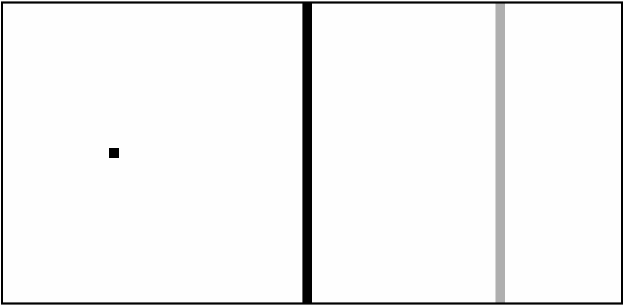
\includegraphics[scale=0.35]{Chapters/Images/synthetic_map.png}
     \caption{}
   \end{subfigure} 
   \begin{subfigure}[c]{.5\linewidth}
     \centering
     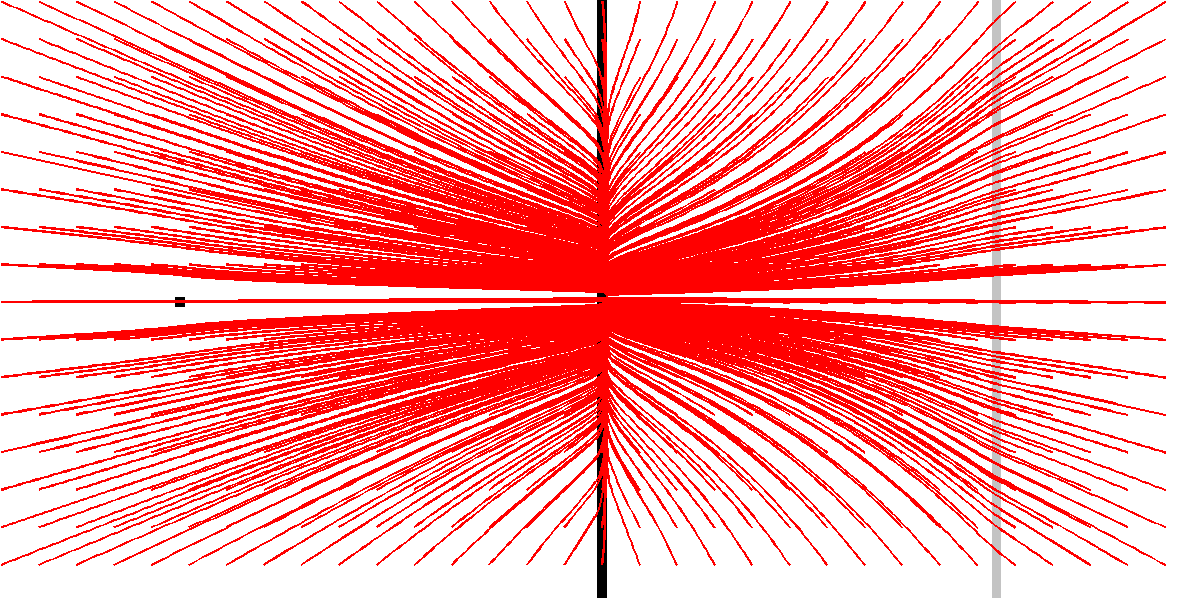
\includegraphics[scale=0.35]{Chapters/Images/m1_gamma_5.png}
     \caption{$\gamma=0.5$}
   \end{subfigure} \\
   
   \begin{subfigure}[c]{.5\linewidth}
     \centering
     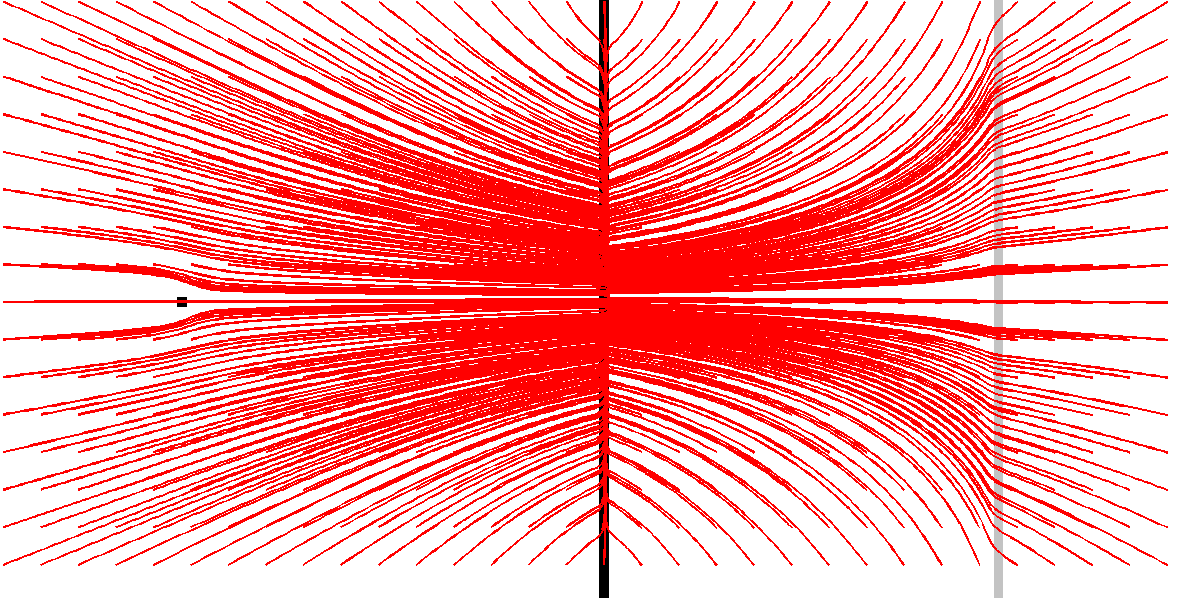
\includegraphics[scale=0.35]{Chapters/Images/m1_gamma_10.png}
     \caption{$\gamma=1.0$}
   \end{subfigure}
   \begin{subfigure}[c]{.5\linewidth}
     \centering
     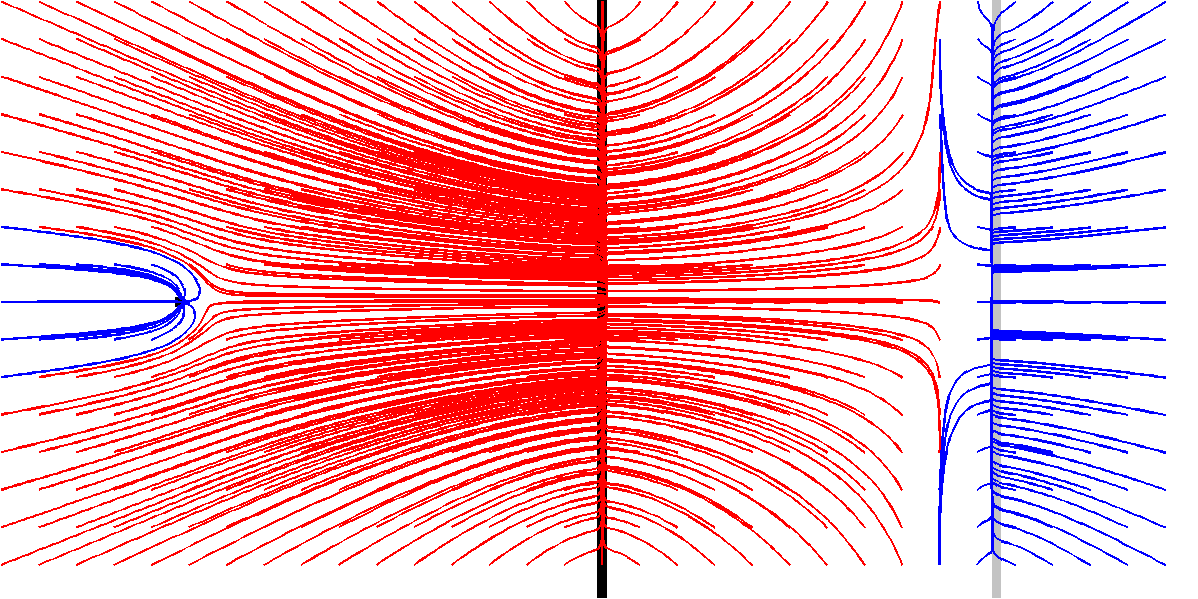
\includegraphics[scale=0.35]{Chapters/Images/m1_gamma_15.png}
     \caption{$\gamma=1.5$}
   \end{subfigure}\\
   
   \begin{subfigure}[c]{.5\linewidth}
     \centering
     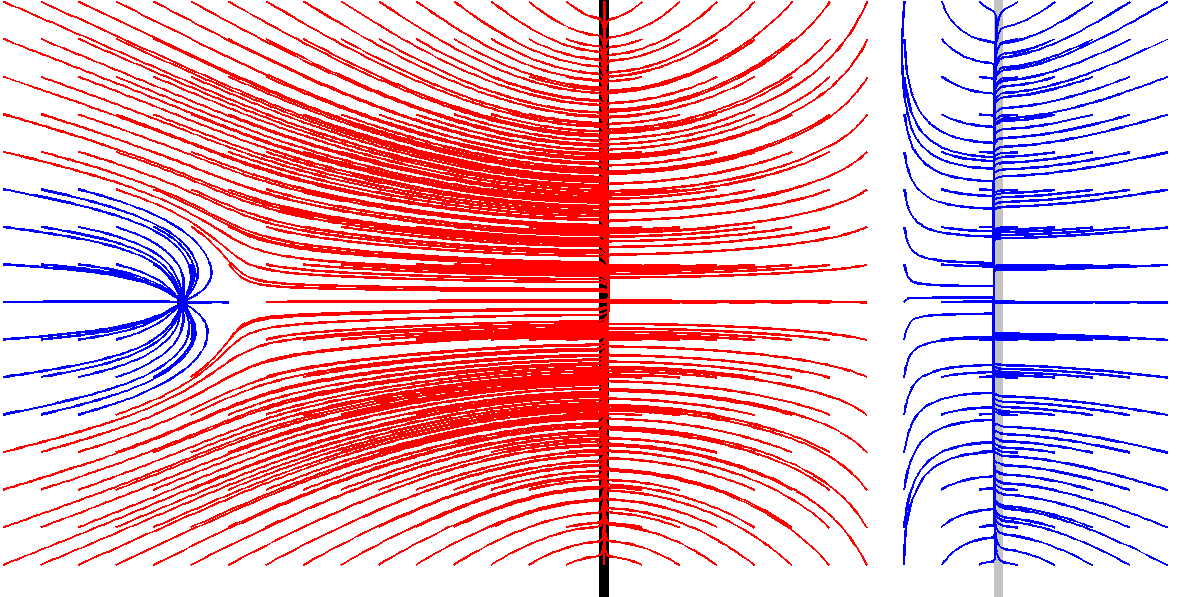
\includegraphics[scale=0.35]{Chapters/Images/m1_gamma_20.png}
     \caption{$\gamma=2.0$}
   \end{subfigure}
   \begin{subfigure}[c]{.5\linewidth}
     \centering
     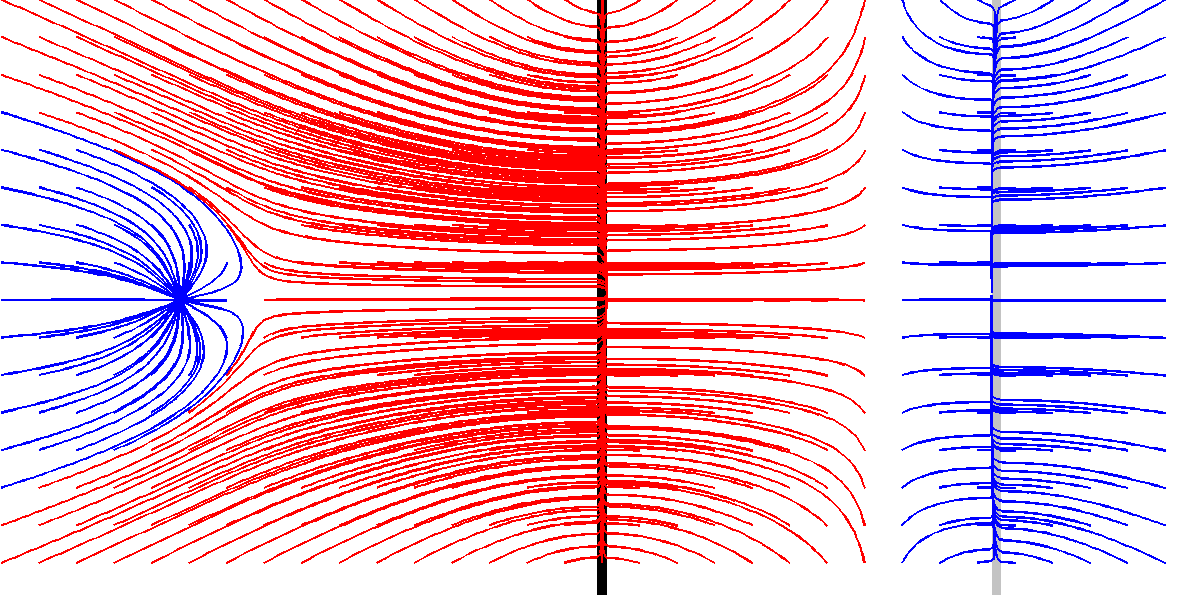
\includegraphics[scale=0.35]{Chapters/Images/m1_gamma_25.png}
     \caption{$\gamma=2.5$}
   \end{subfigure}\\
   
   \caption{(a) Carte de contours $F(x,y)$ synthétique avec un bruit impulsionnel, un contour fort et un contour faible. Lignes de courant générées à partir du champ VFC utilisant $m_1(x,y)$ avec plusieurs valeurs du paramètre $\gamma$ et pour un rayon $R=128$ du noyau de convolution.}
   \label{fig:gamma}
\end{figure}
\subsection{Analyse de $m_1(x,y)$}
\begin{figure}[!h]
   \begin{subfigure}[c]{.5\linewidth}
     \centering
     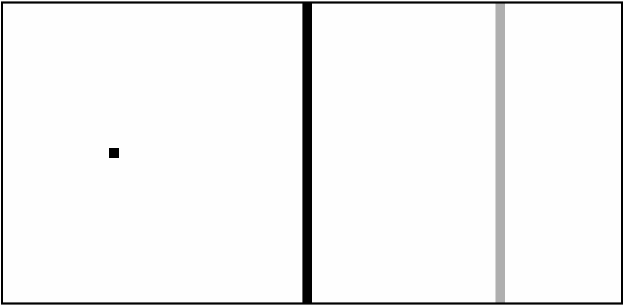
\includegraphics[width=\textwidth]{Chapters/Images/synthetic_map.png}
     \caption{}
   \end{subfigure} 
      \begin{subfigure}[c]{.5\linewidth}
     \centering
     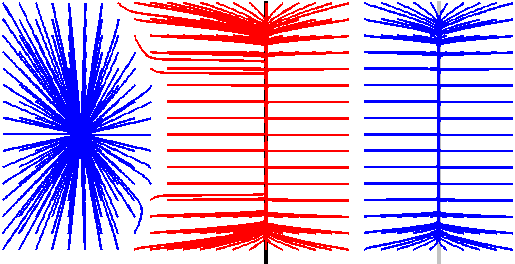
\includegraphics[width=\textwidth]{Chapters/Images/m2_sigma_10.png}
     \caption{$\sigma=10$}
   \end{subfigure} \\
   
   \begin{subfigure}[c]{.5\linewidth}
     \centering
     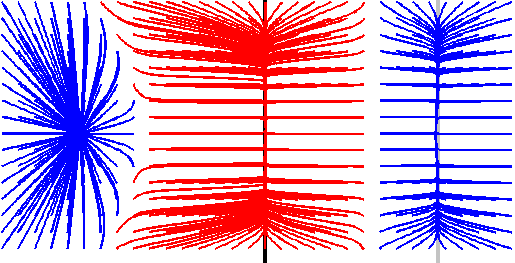
\includegraphics[width=\textwidth]{Chapters/Images/m2_sigma_15.png}
     \caption{$\sigma=15$}
   \end{subfigure}   
   \begin{subfigure}[c]{.5\linewidth}
     \centering
     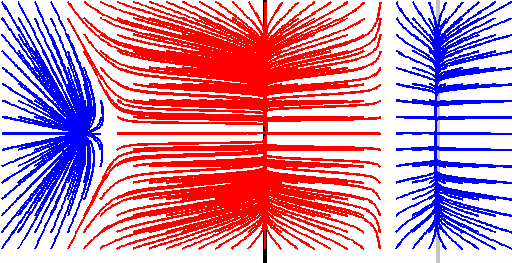
\includegraphics[width=\textwidth]{Chapters/Images/m2_sigma_20.png}
     \caption{$\sigma=20$}
   \end{subfigure}\\
   
   \begin{subfigure}[c]{.5\linewidth}
     \centering
     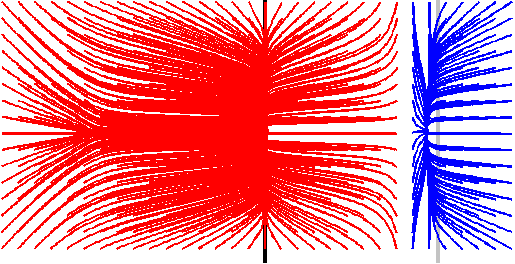
\includegraphics[width=\textwidth]{Chapters/Images/m2_sigma_25.png}
     \caption{$\sigma=25$}
   \end{subfigure}
   \begin{subfigure}[c]{.5\linewidth}
     \centering
     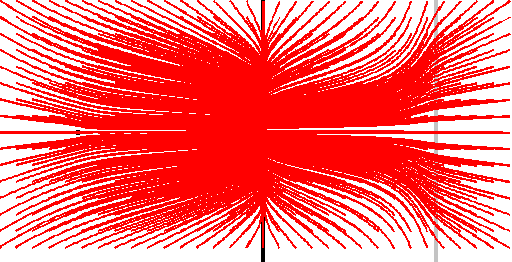
\includegraphics[width=\textwidth]{Chapters/Images/m2_sigma_30.png}
     \caption{$\sigma=30$}
   \end{subfigure}\\
   
<<<<<<< HEAD
   \caption{(a) Carte de contours $F(x,y)$ synthétique avec un bruit impulsionnel, un contour fort et un contour faible. Lignes de courant générées à partir du champ VFC utilisant $m_1(x,y)$ avec plusieurs valeurs du paramètre $\gamma$ .}
   \label{fig:synthetic_map}
\end{figure}

\section{Convergence des concavités}
\begin{figure}[H]

\begin{subfigure}[c]{.5\textwidth}
\centering
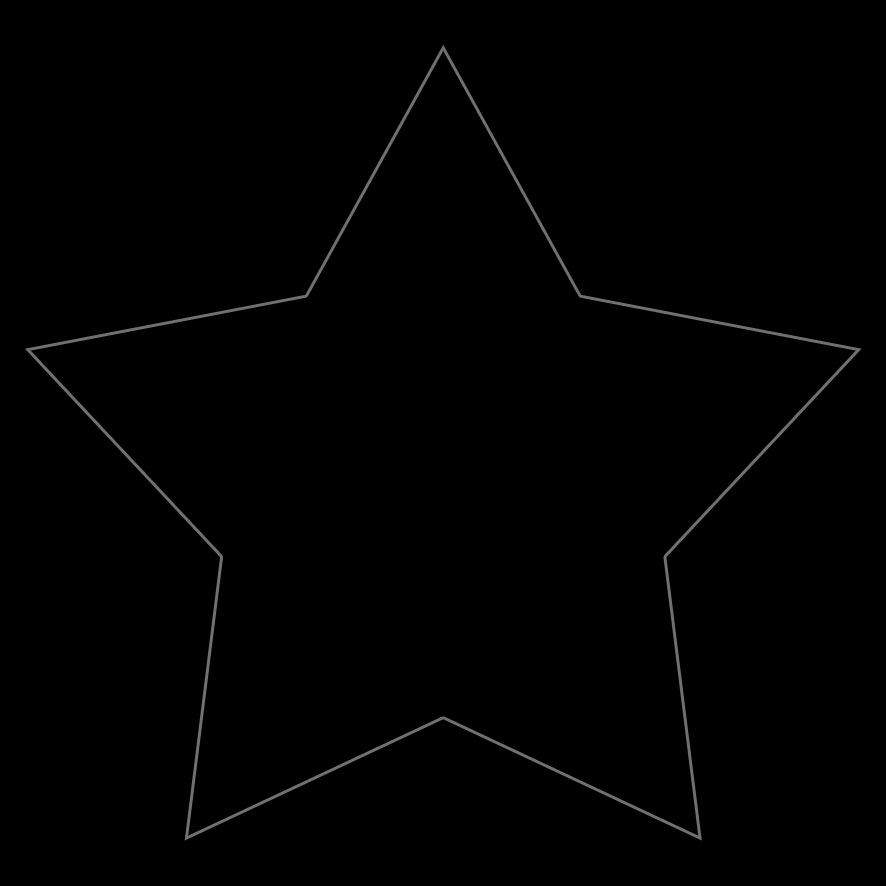
\includegraphics[width=\textwidth]{Images/star}
\caption{}
\end{subfigure}
\begin{subfigure}[c]{.5\textwidth}
\centering
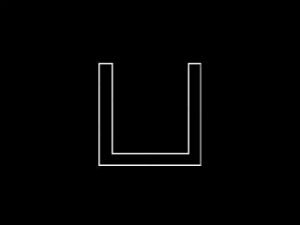
\includegraphics[width=\textwidth]{Images/square}
\caption{}
\end{subfigure}
\caption{Images synthétiques pour les tests de concavités}
\label{fig:ann_synthetic_star_square}
\end{figure}

\begin{figure}[H]
\begin{tabular}{cccc}
\includegraphics[width=0.2\textwidth]{Images/gvf_star_initconv}
&
\includegraphics[width=0.2\textwidth]{Images/gvf_square_initconv}
&
\includegraphics[width=0.2\textwidth]{Images/vfc_star_initconv}
&
\includegraphics[width=0.2\textwidth]{Images/vfc_square_initconv}
\\

\includegraphics[width=0.2\textwidth]{Images/gvf_star_conv}
&
\includegraphics[width=0.2\textwidth]{Images/gvf_square_conv}
&
\includegraphics[width=0.2\textwidth]{Images/vfc_star_conv}
&
\includegraphics[width=0.2\textwidth]{Images/vfc_square_conv}
\end{tabular}
\caption{Initialisation et convergence des contours actifs dans le cas de GVF (deux colonnes de gauche) et de VFC (deux colonnes de droite)}
\label{fig:ann_concavities_results}
\end{figure}

\section{Analyse de l'initialisation du contour actif}

\begin{figure}[H]
\begin{tabular}{cccc}

\includegraphics[width=0.2\textwidth]{Images/vfc_init_centbig}
&
\includegraphics[width=0.2\textwidth]{Images/vfc_init_centsmall}
&
\includegraphics[width=0.2\textwidth]{Images/vfc_init_uncsmall}
&
\includegraphics[width=0.2\textwidth]{Images/vfc_init_uncbig}
\\

\includegraphics[width=0.2\textwidth]{Images/vfc_mid_centbig}
&
\includegraphics[width=0.2\textwidth]{Images/vfc_mid_centsmall}
&
\includegraphics[width=0.2\textwidth]{Images/vfc_mid_uncsmall}
&
\includegraphics[width=0.2\textwidth]{Images/vfc_mid_uncbig}
\\

\includegraphics[width=0.2\textwidth]{Images/vfc_conv_centbig}
&
\includegraphics[width=0.2\textwidth]{Images/vfc_conv_centsmall}
&
\includegraphics[width=0.2\textwidth]{Images/vfc_conv_uncsmall}
&
\includegraphics[width=0.2\textwidth]{Images/vfc_conv_uncbig}
\end{tabular}
\caption{Initialisation, evolution et après 100 itérations. De gauche à droite : Initialisation centrée et grosse, Initialisation centrée petite, Initialisation décentrée petite, Initialisation décentrée et grosse}
\label{fig:ann_init_results}
\end{figure}

\section{Analyse de l'impact du bruit}
\label{fig:ann_noise_results}

\begin{figure}[H]
\begin{subfigure}[c]{.5\textwidth}
\centering
\includegraphics[width=\textwidth]{•}
\caption{}
\end{subfigure}
\begin{subfigure}[c]{.5\textwidth}
\centering
\includegraphics[width=\textwidth]{•}
\caption{}
\end{subfigure}
\caption{GVF ($\mu = 0.2, nb_{iteration} = 10000$) : (a) Bruit gaussien $\sigma = 0.01$, (b) Bruit gaussien $\sigma = 0.15$}
\end{figure}


\begin{figure}[H]
\begin{subfigure}[c]{.5\textwidth}
\centering
\includegraphics[width=\textwidth]{•}
\caption{}
\end{subfigure}
\begin{subfigure}[c]{.5\textwidth}
\centering
\includegraphics[width=\textwidth]{•}
\caption{}
\end{subfigure}
\caption{GVF ($\mu = 0.2, nb_{iteration} = 10000$): (a) Bruit poivre \& sel $0.05\%$, (b) Bruit poivre \& sel $0.10\%$}
\end{figure}


\begin{figure}[H]
\begin{subfigure}[c]{.5\textwidth}
\centering
\includegraphics[width=\textwidth]{•}
\caption{}
\end{subfigure}
\begin{subfigure}[c]{.5\textwidth}
\centering
\includegraphics[width=\textwidth]{•}
\caption{}
\end{subfigure}
\caption{VFC ($R = 128, \gamma = 1.7$) : (a) Bruit gaussien $\sigma = 0.01$, (b) Bruit gaussien $\sigma = 0.5$}
\end{figure}


\begin{figure}[H]
\begin{subfigure}[c]{.33\textwidth}
\centering
\includegraphics[width=\textwidth]{•}
\caption{}
\end{subfigure}
\begin{subfigure}[c]{.33\textwidth}
\centering
\includegraphics[width=\textwidth]{•}
\caption{}
\end{subfigure}
\begin{subfigure}[c]{.33\textwidth}
\centering
\includegraphics[width=\textwidth]{•}
\caption{}
\end{subfigure}



\caption{VFC ($R = 128, \gamma = 1.7$) : (a) Bruit poivre \& sel $0.01\%$, (b) Bruit poivre \& sel $0.05\%$, (c) Bruit poivre \& sel $0.15\%$}
\end{figure}

\begin{figure}[H]
\centering
\includegraphics[width=0.5\textwidth]{•}
\caption{VFC ($R = 64, \gamma = 1.7$) : Bruit gaussien $\sigma = 0.05$  }
\end{figure}
=======
   \caption{(a) Carte de contours $F(x,y)$ synthétique avec un bruit impulsionnel, un contour fort et un contour faible. Lignes de courant générées à partir du champ VFC utilisant $m_2(x,y)$ avec plusieurs valeurs du paramètre $\sigma$ et pour un rayon $R=128$ du noyau de convolution.}
   \label{fig:sigma}
\end{figure}
>>>>>>> b8de5ad016d126a3298c5e56452deb919677aab8
